\section{Functionalities of the System}

In this chapter,
we introduce two interactive mockups of our disaster monitoring model.
The first mockup is built for game players,
which is used for collecting human inputs.
The second mockup is built for some collaborative organisations,
such as Unicef and some NGOs,
who wants to dispatch their rescue teams in disaster area more properly. 

  \subsection{Functionalities as Seen by a Player}
      \subsubsection{Disaster Monitoring Game Introduction}
      The idea behind our human computation system is GWAP,
      that is Game With a Purpose.
      We have sketched a mockup of image tagging game,
      which is similar to the ESP game on Artigo.com \cite{wieser2013artigo}.
      In our game,
      A player can finish infinity round tasks, 
      a Round task contains $N$ tagging tasks and a tagging task is to:
      interpret one picture.
      Within one round task, the player will see $N$ pictures.
      Each time he/she will be asked to tag one of these pictures.
      At first,
      the player needs to draw a rectangle area which indicates that he/she has seen some objects in this area.
      Thoses objects are often considered as a sign of danger or damage.
      They are mostly like:
      
      \begin{itemize}
        \item ``Rocket Launcher''
        \item ``Armoured vehicles''
        \item ``Tanks''
        \item ``Burning building''
        \item ``Heavy vehicle tracks''
        \item ``sign of explosion''
      \end{itemize}

      Each of them has a value of disaster level, 
      which will be used later in our (see chapter \ref{chapter:dem}) for analysing the disaster level of this region.
      A submenu list (``Pre-provided item list'') which contains all of these items will pop up after the area has been selected.
      In this step,
      the player can decide which one of these items matches and then choose it.
      The player can also obtain helps from the reference panel which provides the player with examples.
      Besides, 
      if the player does not find the expected item in the ``Pre-Provided item list'',
      he/she can also create a new tag.

      In a tagging task,
      the player also has a choice to add multiple tags to one picture,
      or he/she dosen't need to add any tags when he/she thinks that this region is safe.

      After finishing one tagging task, 
      the player will be directed to the next task till the end of the game.


      \subsubsection{Examples}
      In this section,
      An example of a user journey is provided in order to illustrate the game process.

      \noindent\begin{minipage}{.45\textwidth}
      \begin{figure}[H]
      \centering
      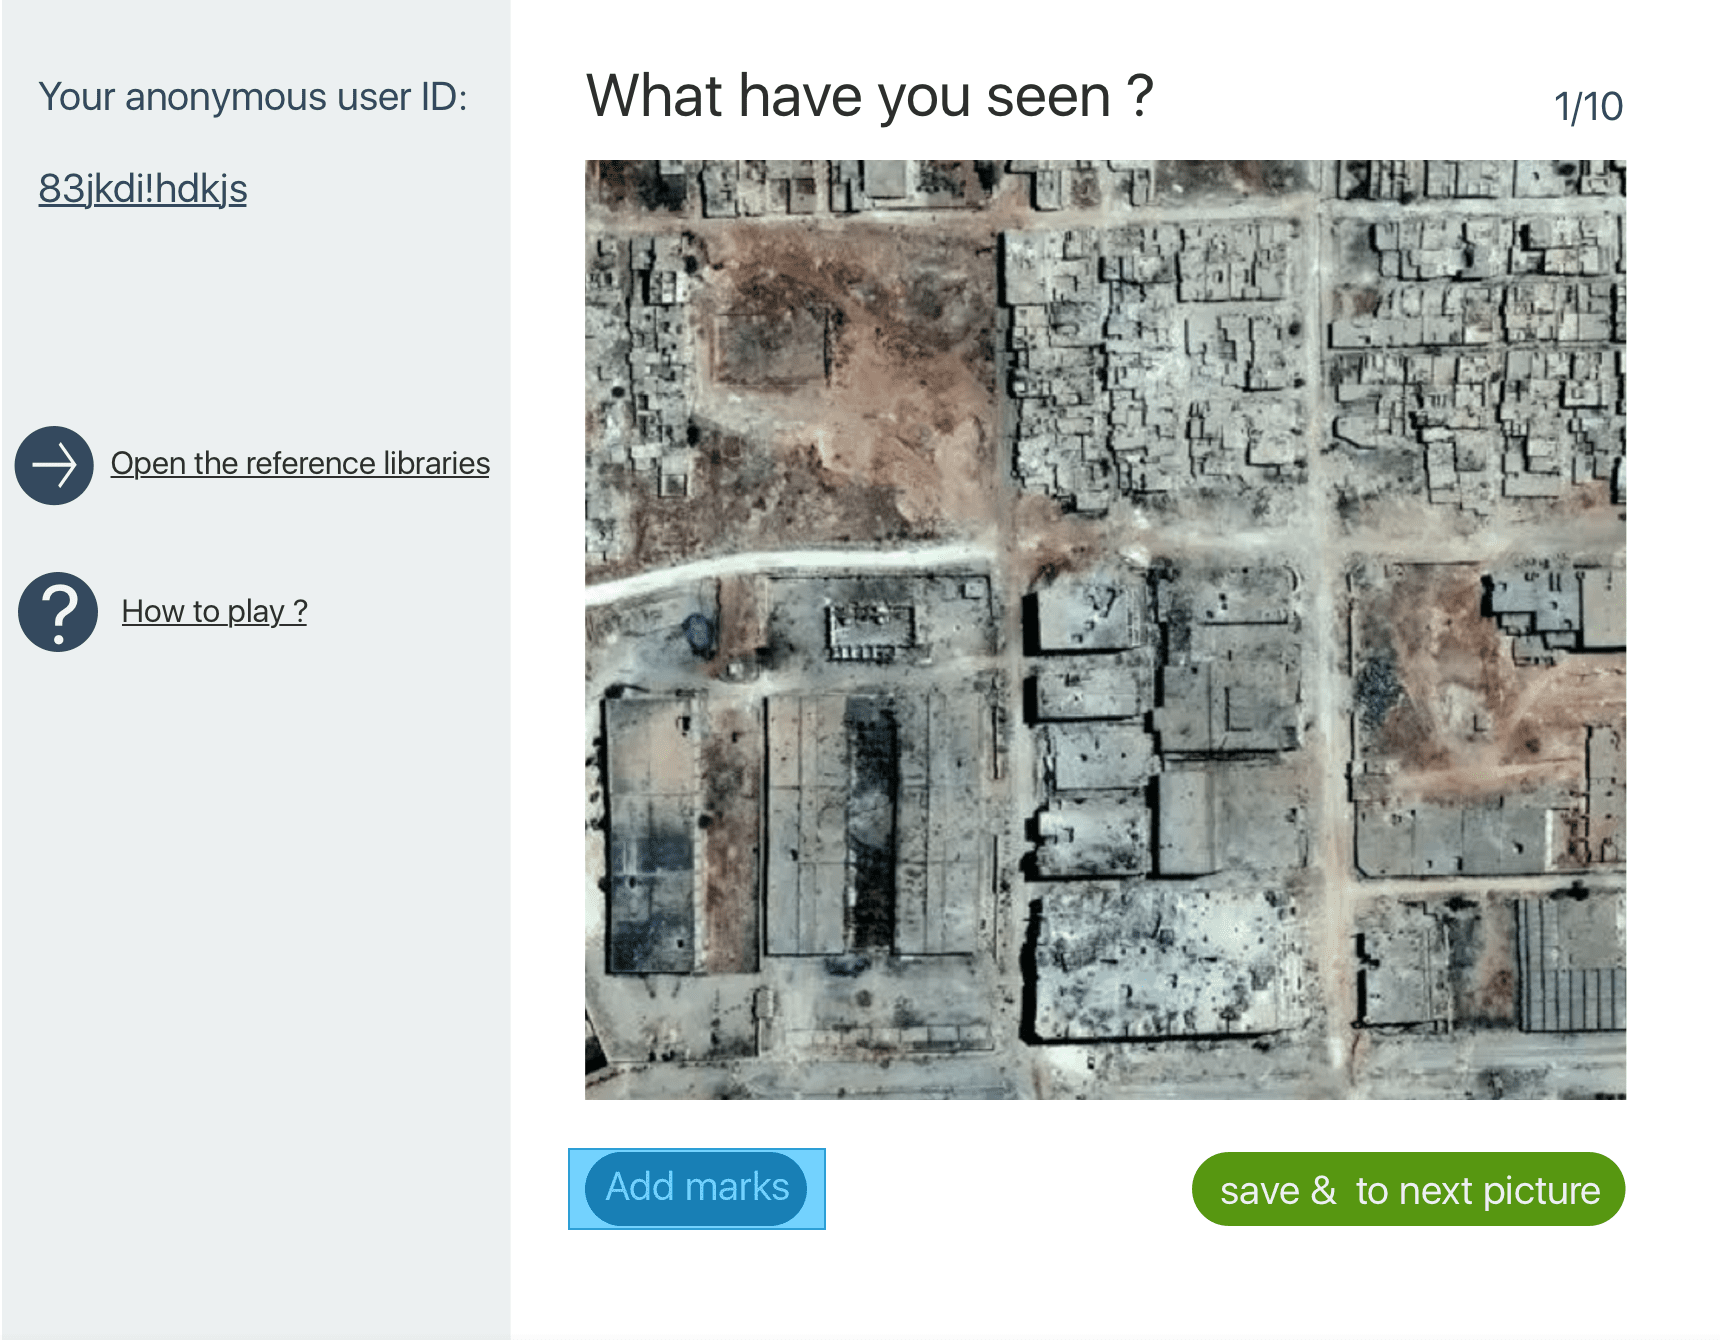
\includegraphics[width=\textwidth]{figures/function-player-0}
      \caption{Game panel\cite{satellite-photo-1}}
      \label{fig:player0}
      \end{figure}
      \end{minipage}\hfill
      \noindent\begin{minipage}{.45\textwidth}
      \begin{figure}[H]
      \centering
      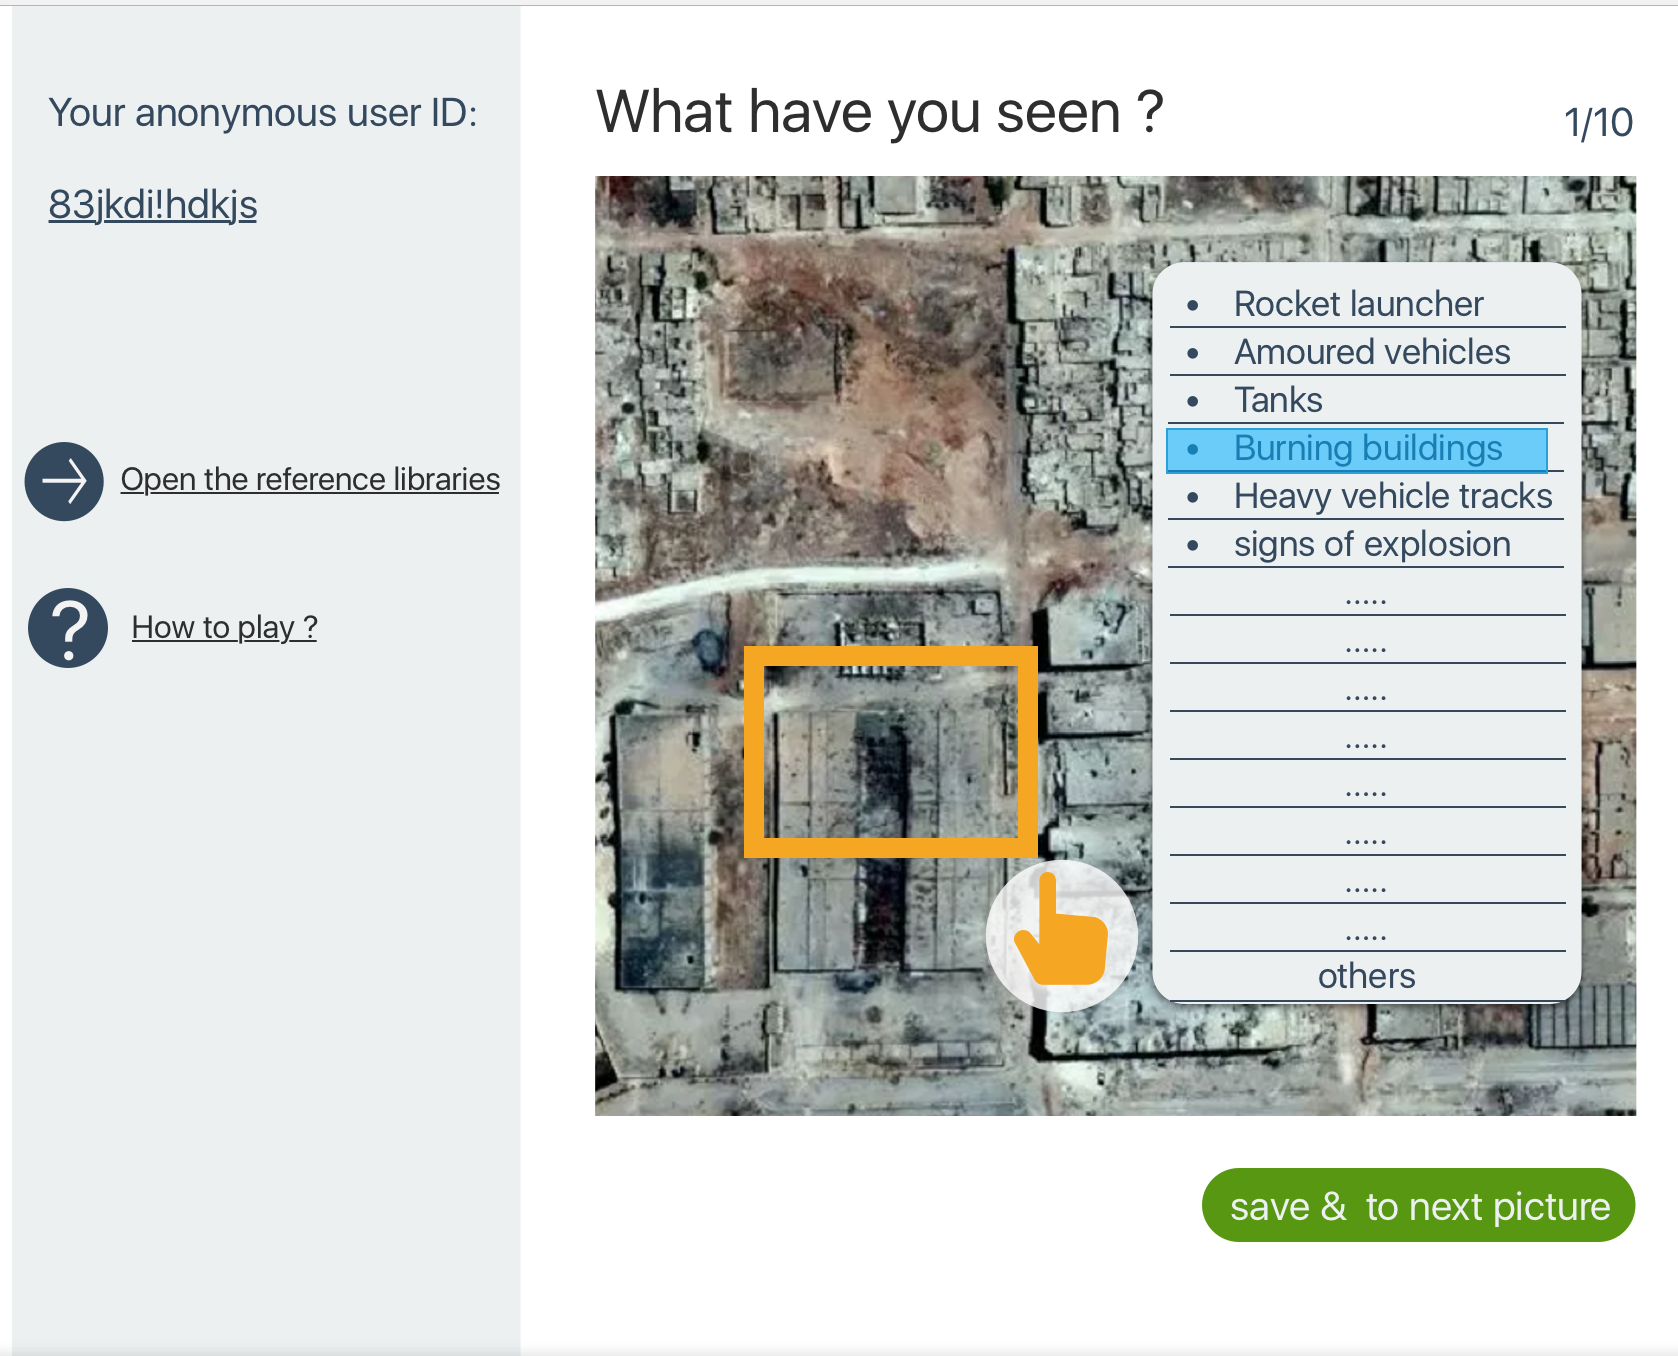
\includegraphics[width=\textwidth]{figures/function-player-1}
      \caption{Game panel: Tag list\cite{satellite-photo-1}}
      \label{fig:player1}
      \end{figure}
      \end{minipage}\hfill

      Imaging that user A is now at the very first begining of the game.
      What he will see,
      are a side bar on the left side,
      which contains some information like:
      user ID,
      game guide and a reference library,
      and a main panel on the right side (Figure \ref{fig:player0}).
      If user A finds a sign of damage or danger in the picture on the right side.
      He can click the button ``add marks'' and then hs is able to draw a rectangle area which indicates the location of the sign.
      A selection box will then pop out automatically and user A can select the suited item or add a new tag (Figure \ref{fig:player1}).

      As already mentioned above,
      user A can also add multiple tags to one picture (Figure \ref{fig:player2}).

      \noindent\begin{minipage}{.45\textwidth}
      \begin{figure}[H]
      \centering
      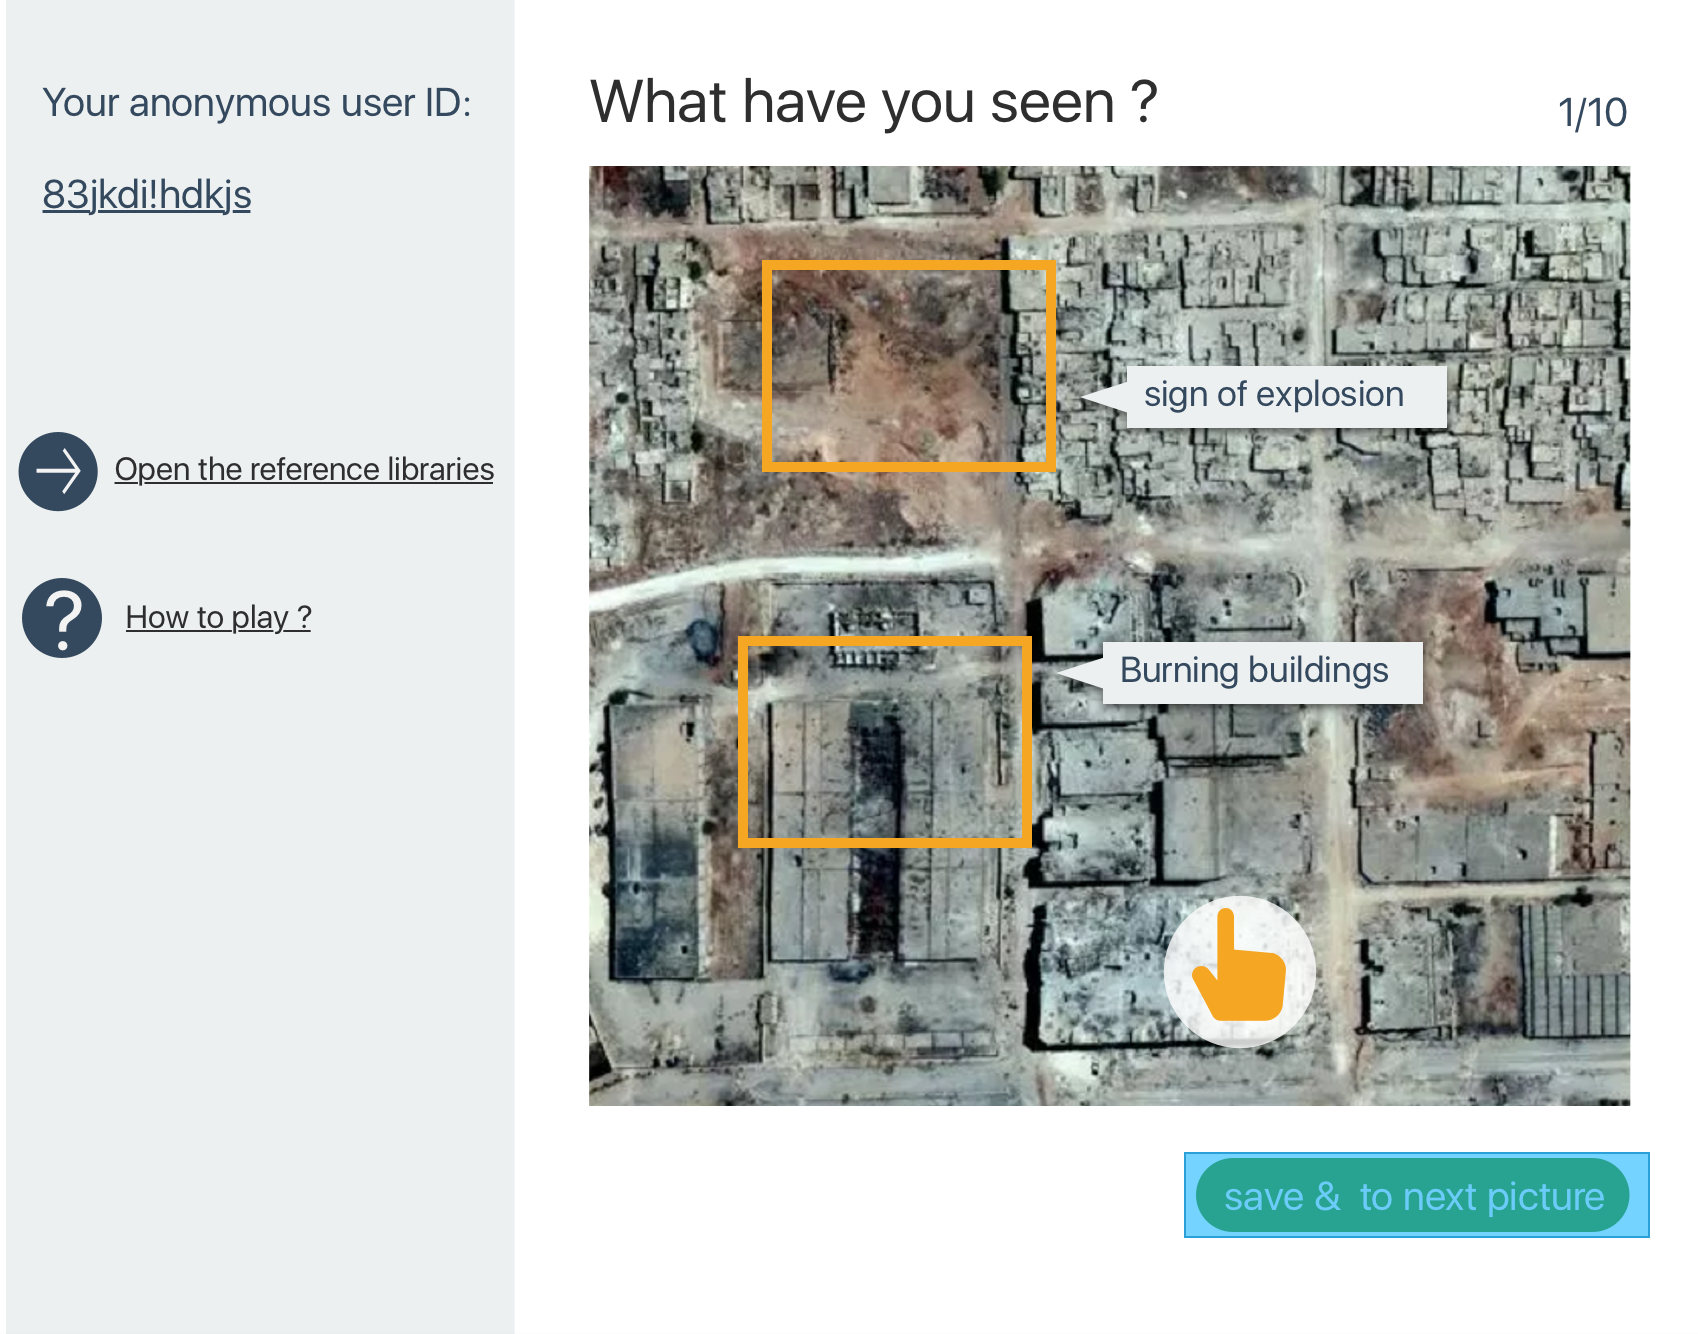
\includegraphics[width=\textwidth]{figures/function-player-2}
      \caption{Game panel: Multiple tags\cite{satellite-photo-1}}
      \label{fig:player2}
      \end{figure}
      \end{minipage}\hfill
      \noindent\begin{minipage}{.45\textwidth}
      \begin{figure}[H]
      \centering
      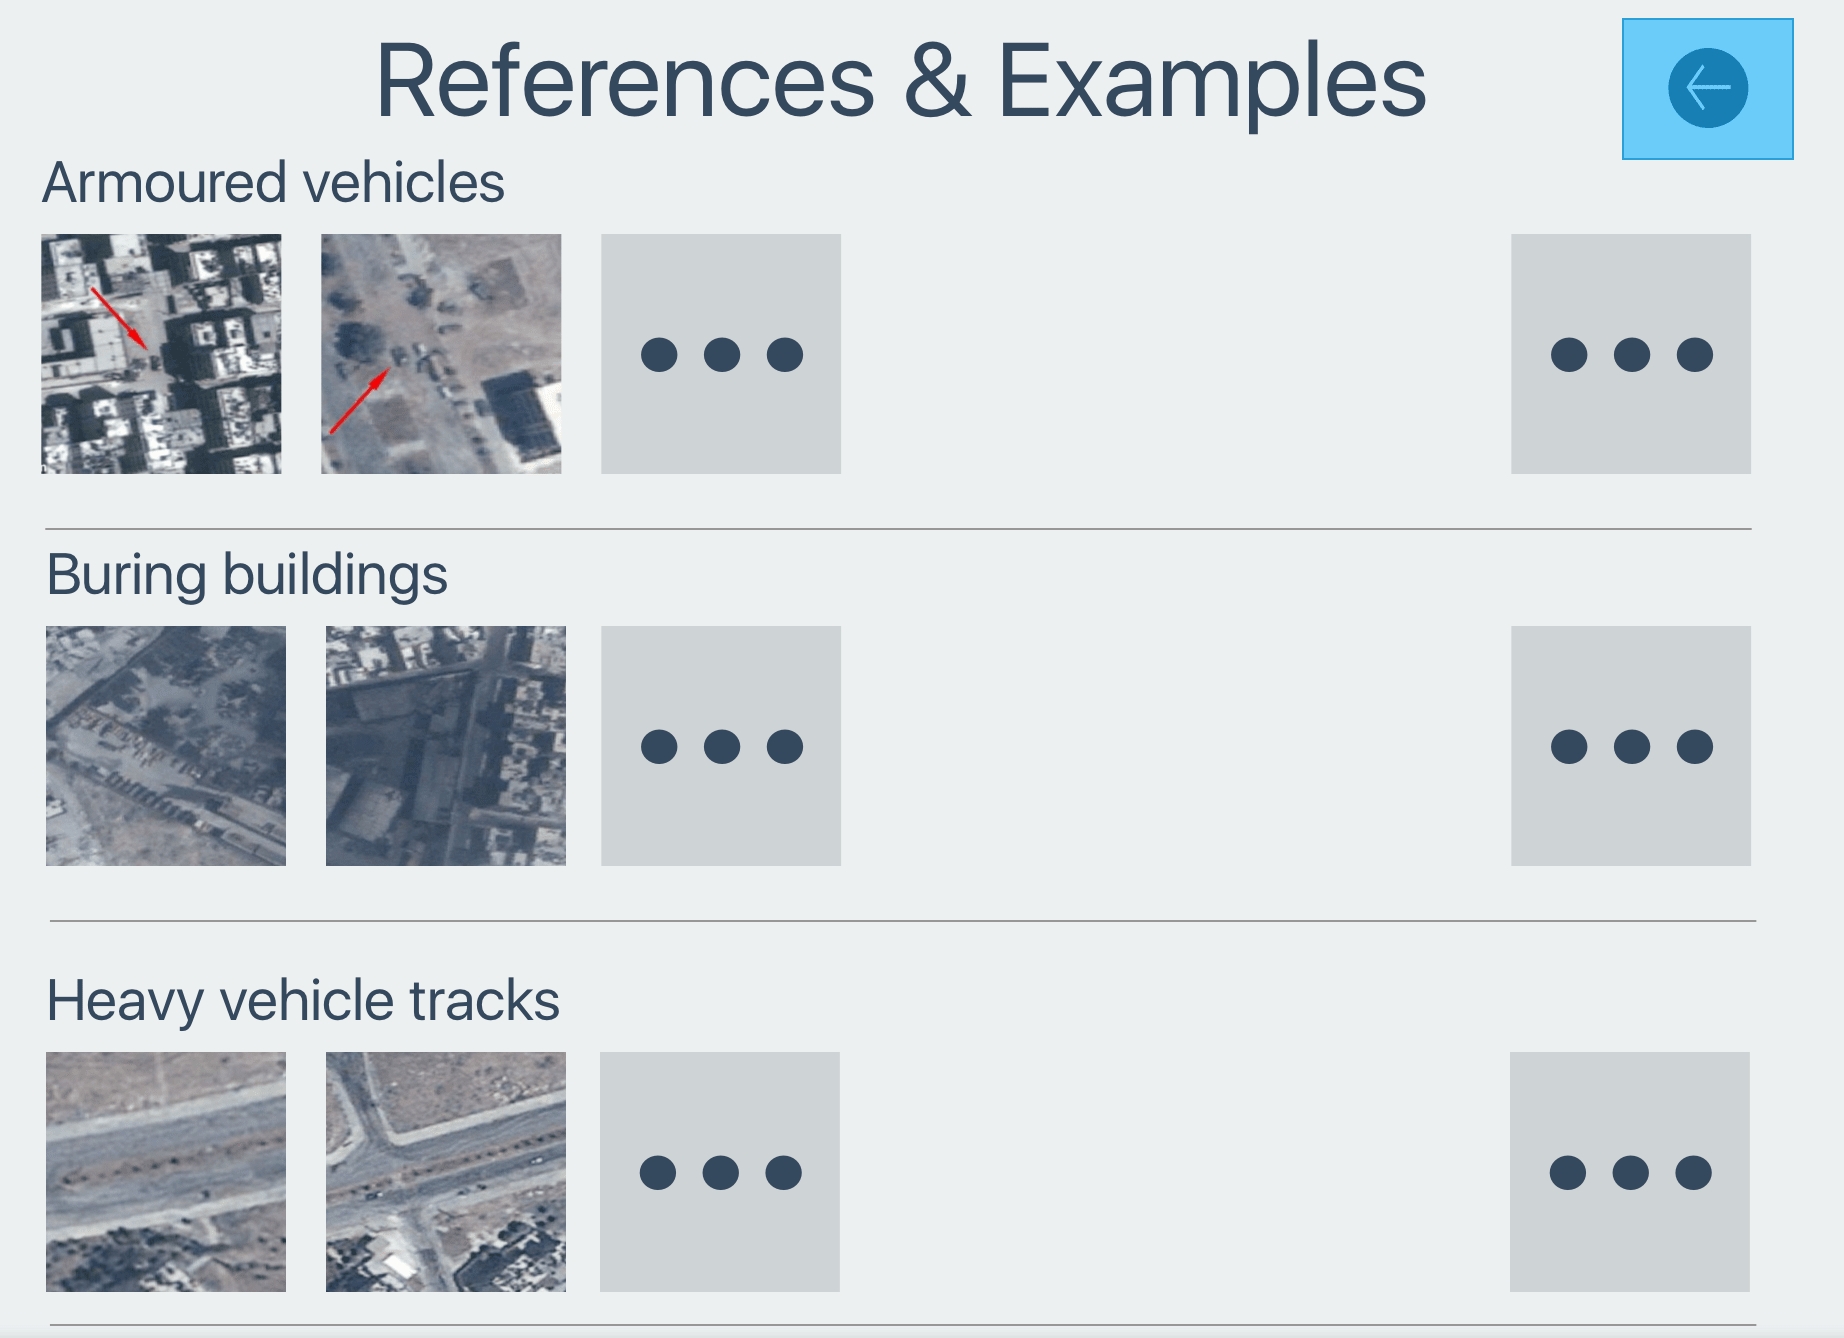
\includegraphics[width=\textwidth]{figures/function-player-3}
      \caption{Game panel: Reference library. Image \textcopyright DigitalGlobe, Inc}
      \label{fig:player3}
      \end{figure}
      \end{minipage}\hfill

      After user A finishes this tagging task,
      i.e.
      tagging the first picture,
      he can click the button "save and to the next picture" so that he can save the tags and go to the next task.
      Figure \ref{fig:player3} illustrates how a reference library can be,
      whose aim is to help user A to identify different signs of danger or damage.

    \subsection{Functionalities as Seen by a Stakeholder}
      In our disaster monitoring system, 
      we take image taggings from players as our input. 
      In the next step, 
      we will filter and analyse the data.
      The final output of our work is a disaster level report in some certain region,
      which can be used by some organasitions,
      like: Unicef, some NGOs and even governments.

      Under this consideration, 
      we also sketched a mockup for this user group,
      which gives them an overview of the disaster level and to download the report at the same time (see figure \ref{fig:stakeholder1}).

      \noindent\begin{minipage}{.45\textwidth}
      \begin{figure}[H]
      \centering
      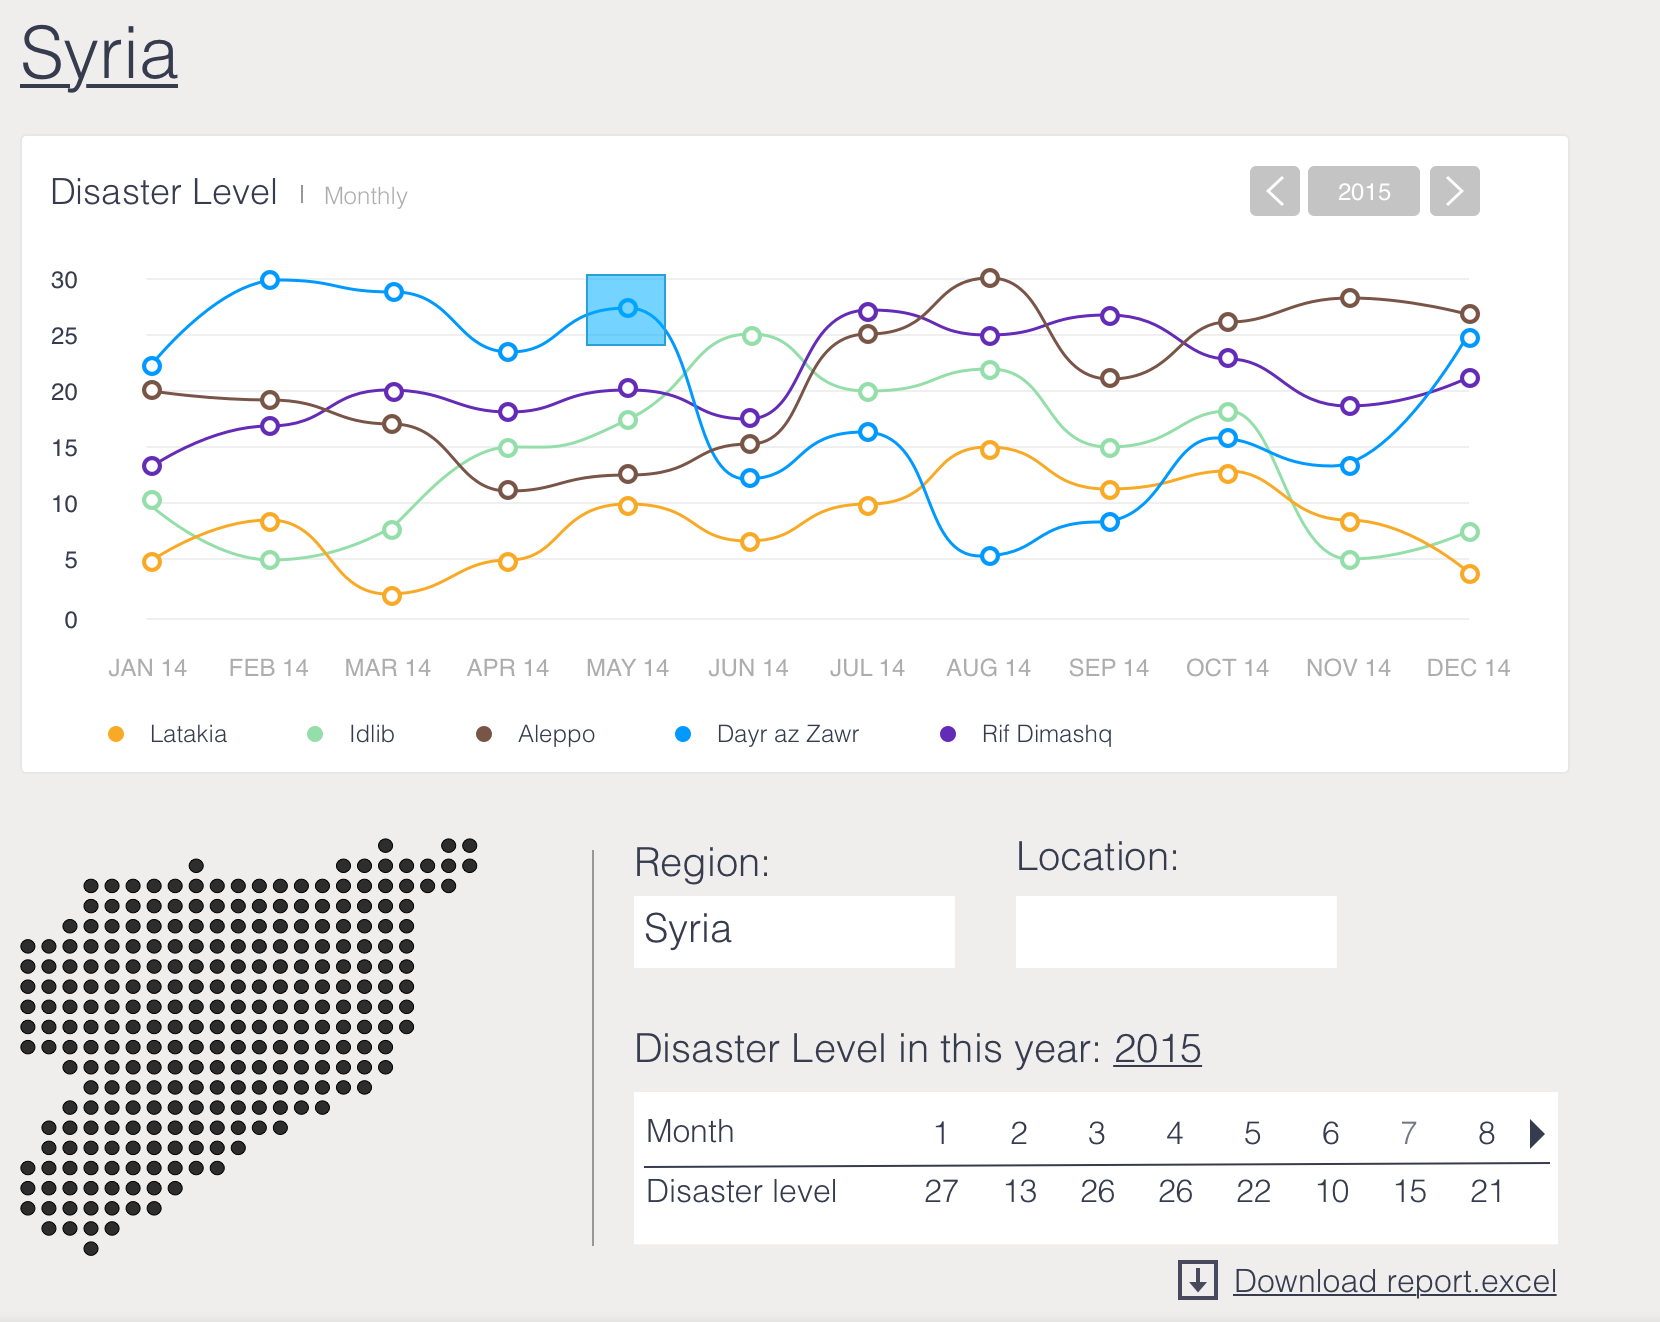
\includegraphics[width=\textwidth]{figures/function-stakeholder-1}
      \caption{disaster level report platform}
      \label{fig:stakeholder1}
      \end{figure}
      \end{minipage}\hfill
      \noindent\begin{minipage}{.45\textwidth}
      \begin{figure}[H]
      \centering
      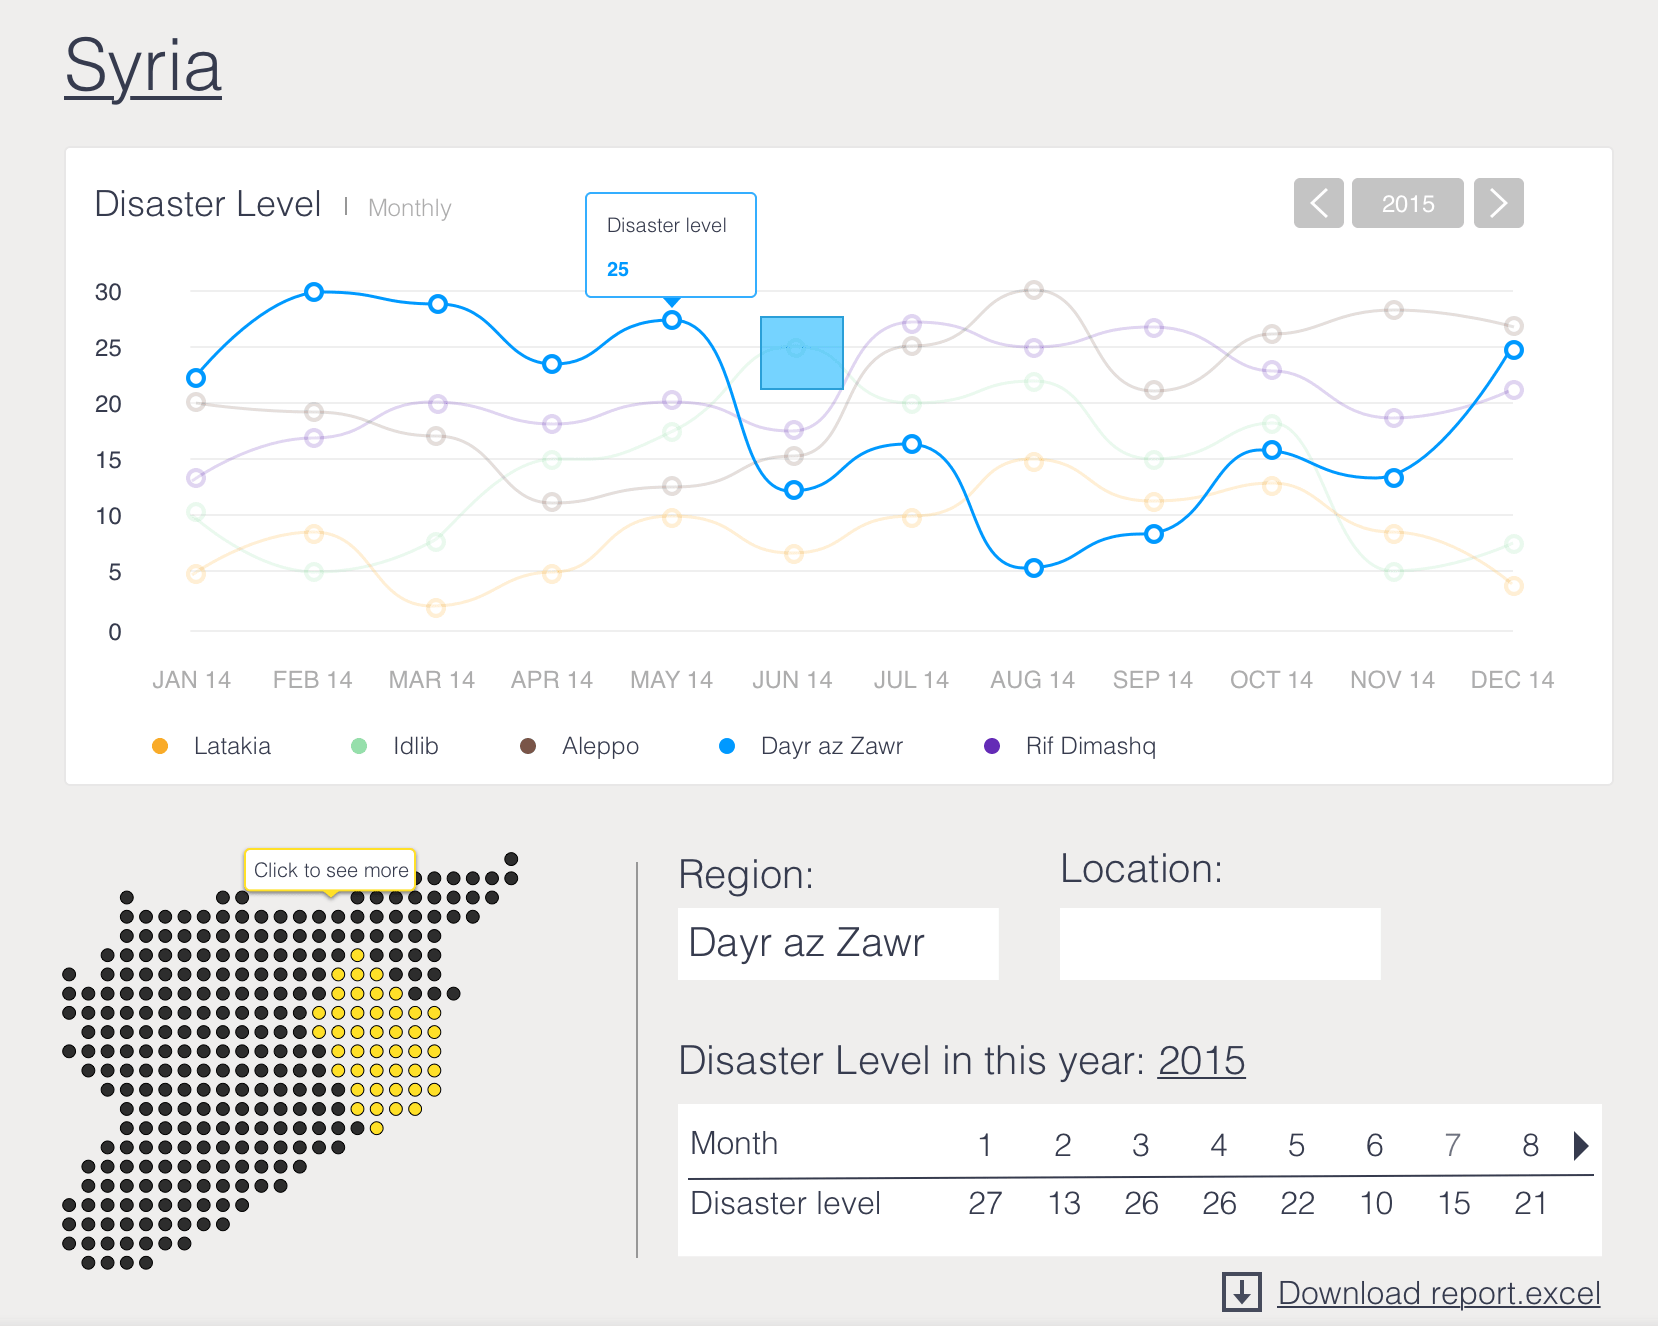
\includegraphics[width=\textwidth]{figures/function-stakeholder-2}
      \caption{disaster level report platform}
      \label{fig:stakeholder2}
      \end{figure}
      \end{minipage}\hfill

      The platform is composed of a curve chart,
      a map and some statistics.
      In the curve chart,
      each curve shows the the yearly disaster level of a smaller region.
      Like here in figure \ref{fig:stakeholder1}, 
      the whole region is Syria and each curve stands for a province in Syria.
      The user can click the "dot" on curves,
      which stands for the disaster level of that month.
      Meanwhile, the corresponding area will be highlighted on the map (figure \ref{fig:stakeholder2}).

      In the statistic part,
      the user gets an overview of the yearly disaster level of a region.
      He/she also have the opportunity to download it.
      If the user wants to dig deeper, 
      he/she can click on the highlighted area on this map,
      which will direct him/her to that region (figure \ref{fig:stakeholder3}).

      \begin{figure}[H]
      \centering
      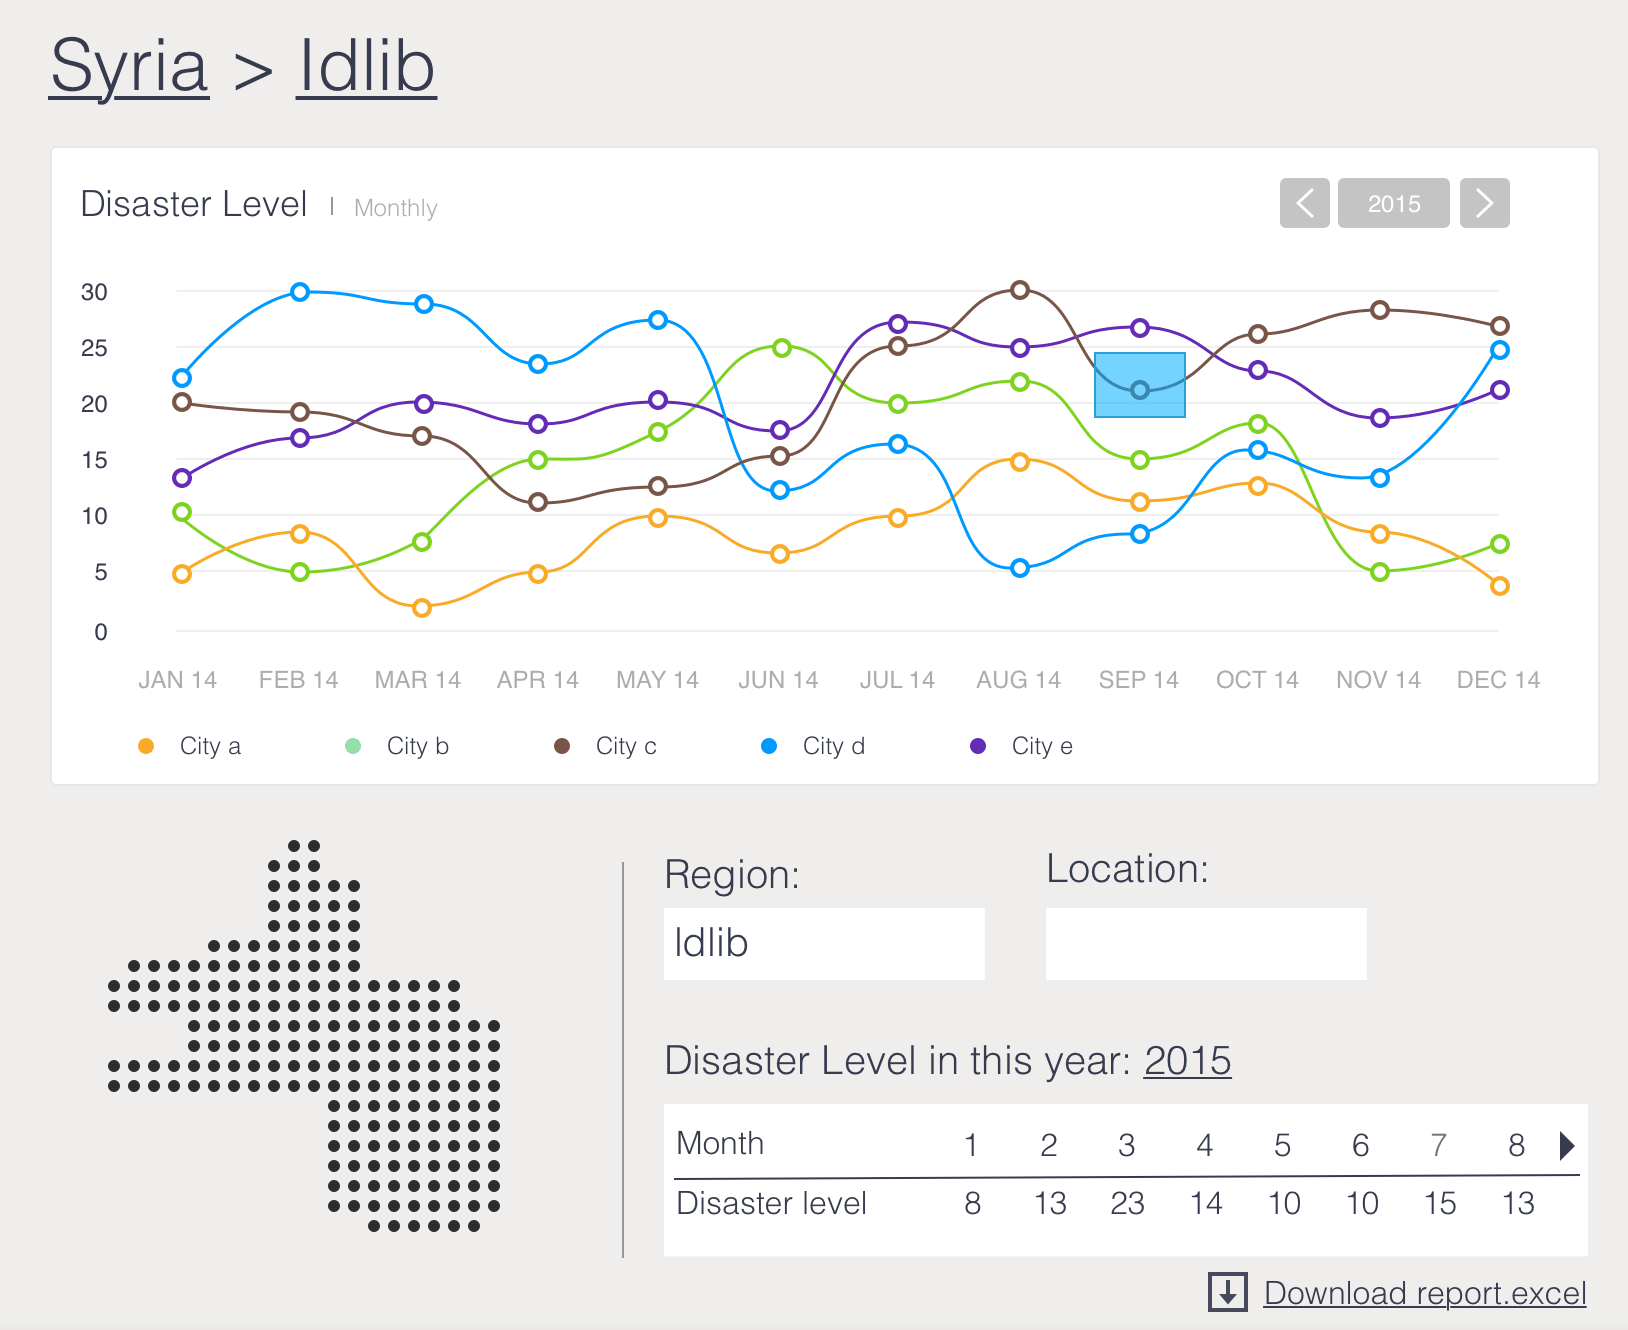
\includegraphics[width=0.5\textwidth]{figures/function-stakeholder-3}
      \caption{Disaster Level Report Platform}
      \label{fig:stakeholder3}
      \end{figure}

      In figure \ref{fig:stakeholder3},
      the user is directed to the province ldlib and now each curve stands for a smaller region in this province,
      in other words, different cities in ldlib.
    
    \subsection{Possible Technology Stack for Implementation}
    In this section, we will discuss the of the future implementation of our system. 

    We suggest to build our system sketched above as a web-based application so that we do not need to care about the platform.
    Our system should be capable of easily acessing by both android users and IOS users. We suggest to choose \textbf{Polymer}, a Google front-end framework, as our front-end tool and as back-end tool, we suggest to use \textbf{Nodejs} and \textbf{Python}. For our databse, we suggest then to choose \textbf{Mango DB}, since it is more suitable for a web-application.